\documentclass[Space3_Assign3.tex]{subfile}

\begin{document}

\begin{figure}[h]
\centering
\caption{Output from Section \fullref{Sec:gengrid}. The start node is in blue and the goal node is in red}
\label{Fig:gengrid}
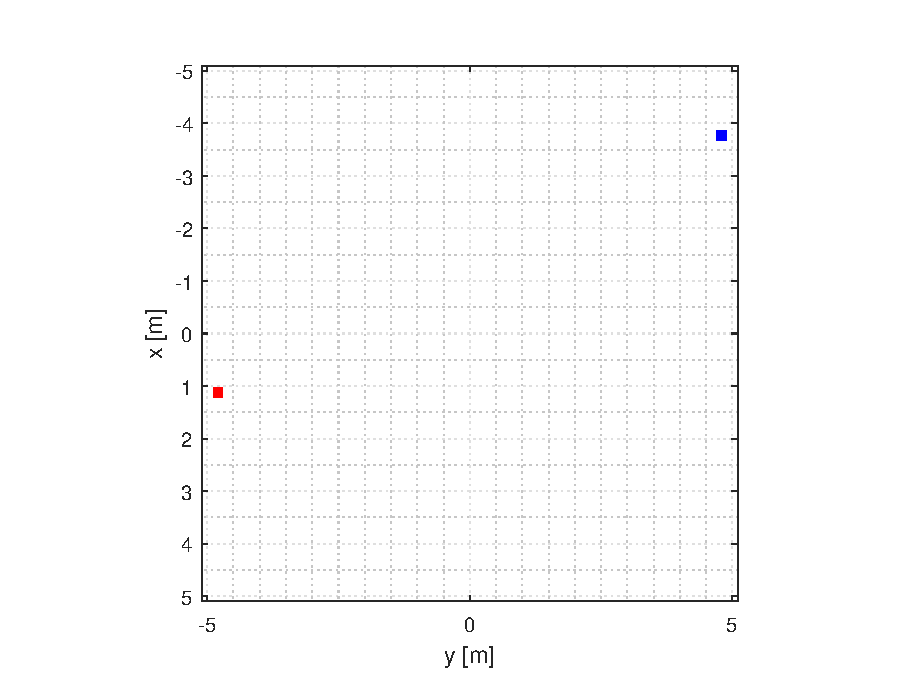
\includegraphics[width = 0.7\linewidth]{generategrid.eps}
\end{figure}

\begin{figure}[h]
\centering
\caption{Output from Section \fullref{Sec:genobs}. The start node is in blue, the goal node is in red and obstacles are black}
\label{Fig:genobs}
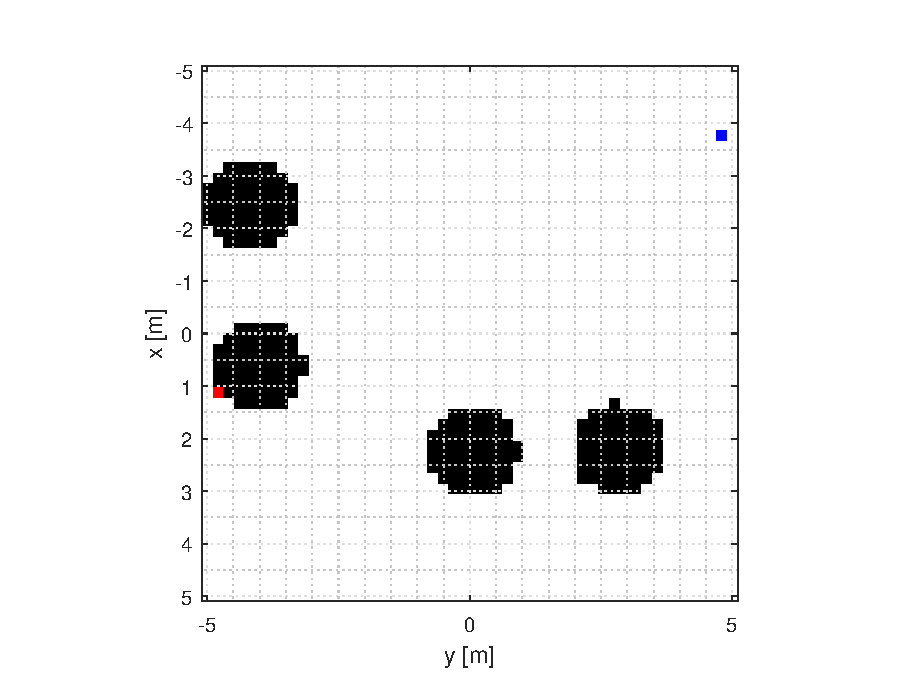
\includegraphics[width = 0.7\linewidth]{generateobstacles.eps}
\end{figure}

\begin{figure}[h]
\centering
\caption{Output from Section \fullref{Sec:trav}. Traversability map: Darker colours indicate a higher cost to travel over. White indicates the rover is unable to travel over.}
\label{Fig:trav}
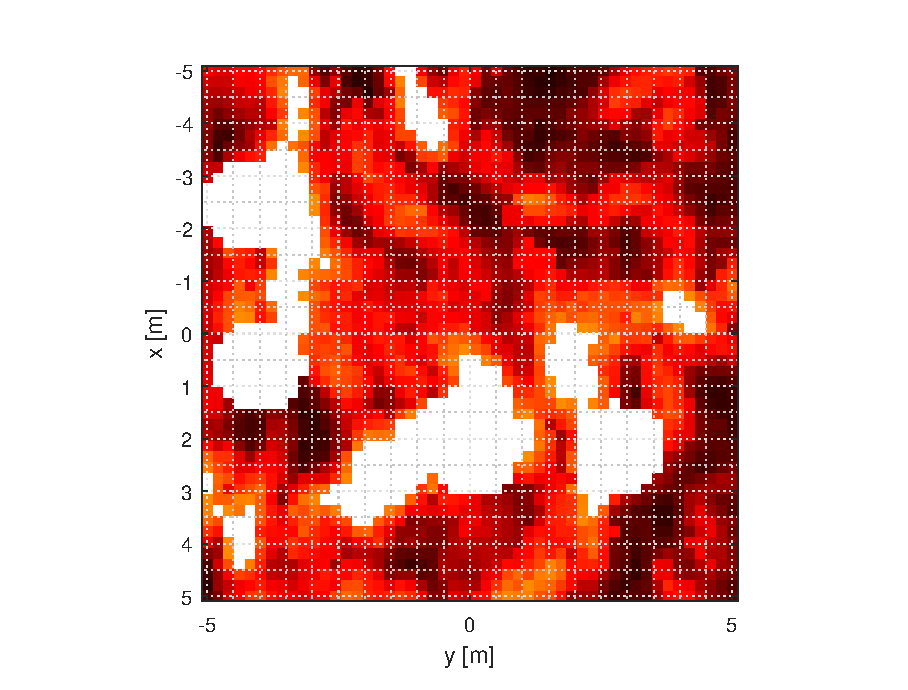
\includegraphics[width = 0.7\linewidth]{trav.eps}
\end{figure}

\begin{figure}[h]
\centering
\caption{Output from Section \fullref{Sec:Dij}. The start node is in blue, the goal node is in red and obstacles are black}
\label{Fig:Dijkstra Algorthim}
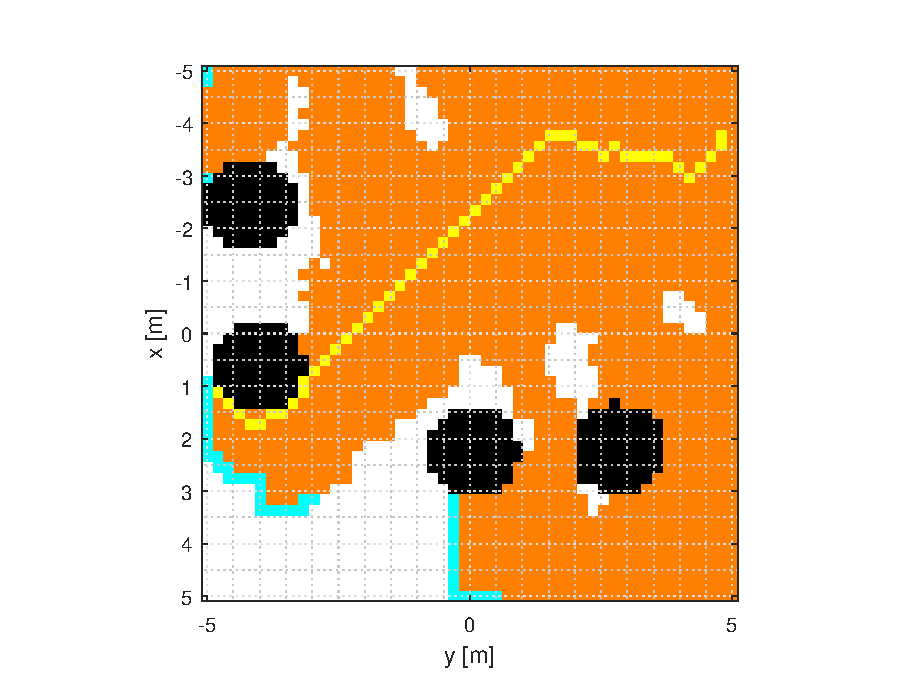
\includegraphics[width = 0.7\linewidth]{DijkstraMap.eps}
\end{figure}

\begin{figure}[h]
\centering
\caption{Output from Section \fullref{Sec:terrain}. }
\label{Fig:DijkstraTerrain}
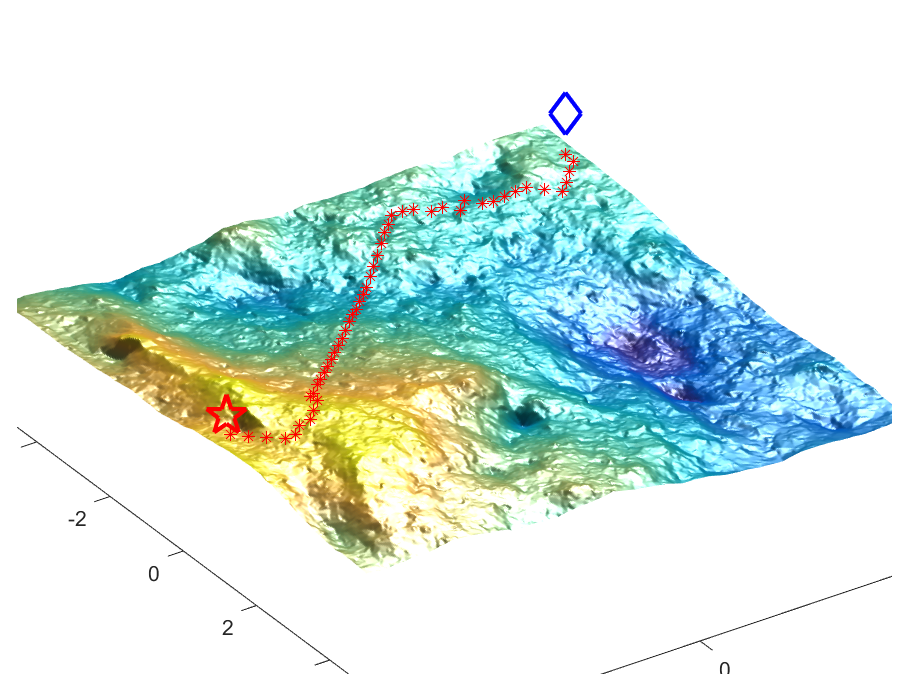
\includegraphics[width = 0.7\linewidth]{Dijstra_terrain.eps}
\end{figure}


\begin{figure}
\centering
\caption{A* Euclidean Distance}
\label{Fig:A*eu}
\begin{subfigure}{0.49\linewidth}
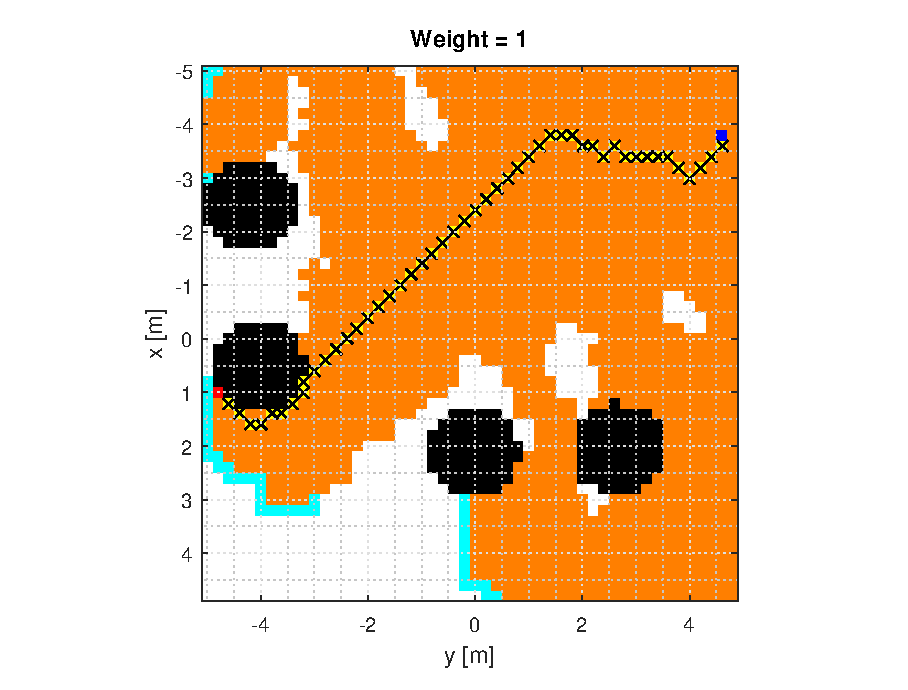
\includegraphics[width = 1\linewidth]{Astar_euc_1.eps}
\end{subfigure}
\begin{subfigure}{0.49\linewidth}
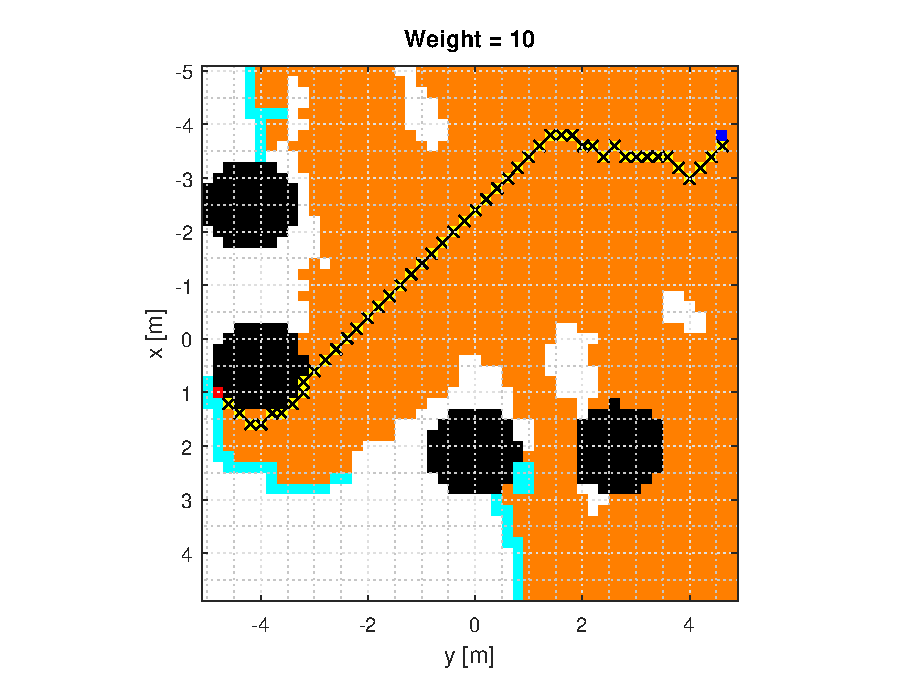
\includegraphics[width = 1\linewidth]{Astar_euc_10.eps}
\end{subfigure}
\begin{subfigure}{0.49\linewidth}
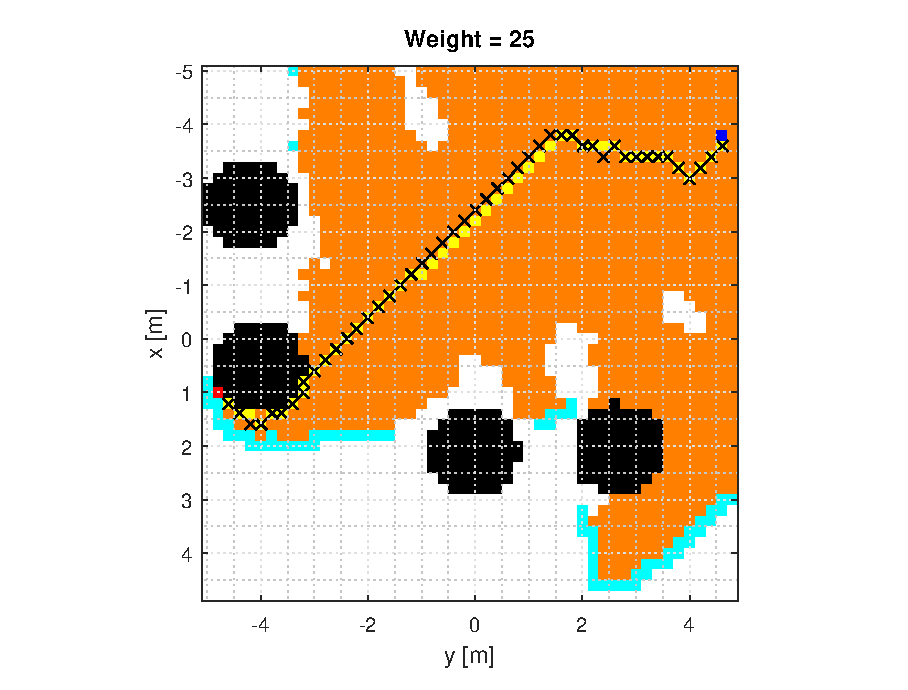
\includegraphics[width = 1\linewidth]{Astar_euc_25.eps}
\end{subfigure}
\begin{subfigure}{0.49\linewidth}
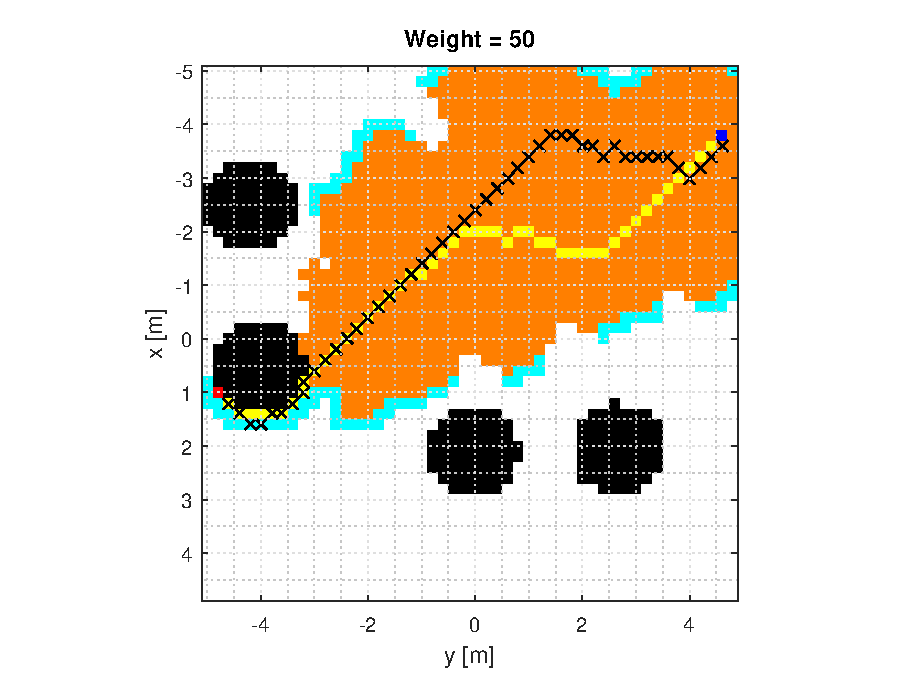
\includegraphics[width = 1\linewidth]{Astar_euc_50.eps}
\end{subfigure}
\begin{subfigure}{0.49\linewidth}
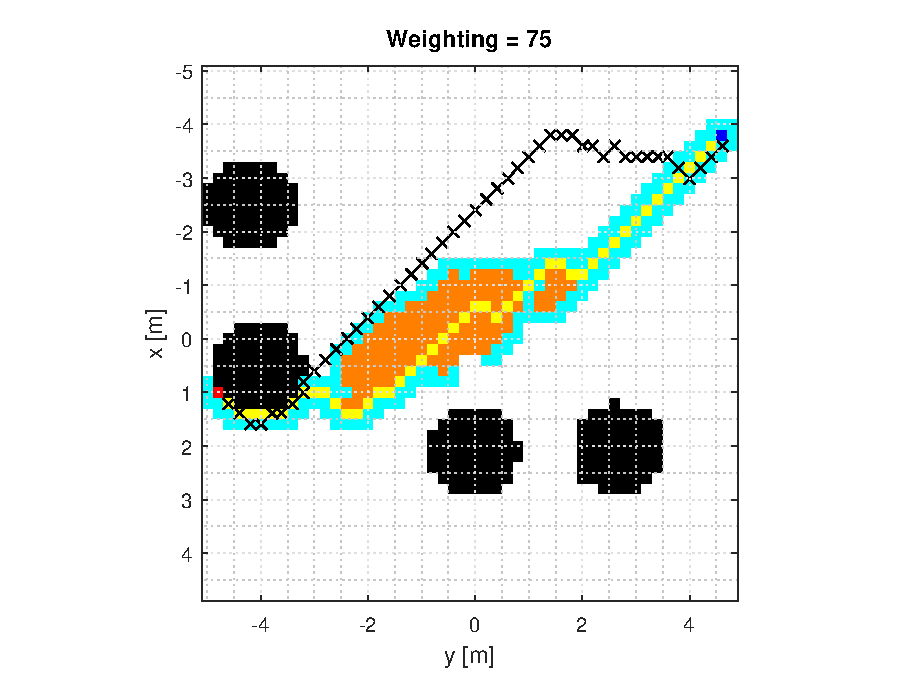
\includegraphics[width = 1\linewidth]{Astar_euc_75.eps}
\end{subfigure}
\begin{subfigure}{0.49\linewidth}
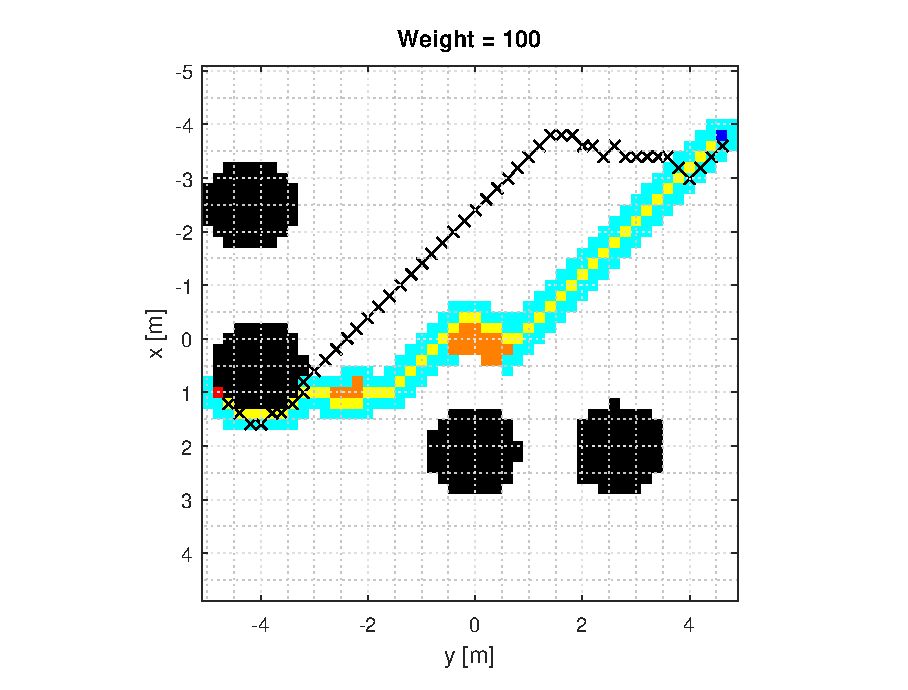
\includegraphics[width = 1\linewidth]{Astar_euc_100.eps}
\end{subfigure}
\end{figure}

\begin{figure}
\centering
\caption{A* Manhattan Distance}
\label{Fig:A*eu}
\begin{subfigure}{0.49\linewidth}
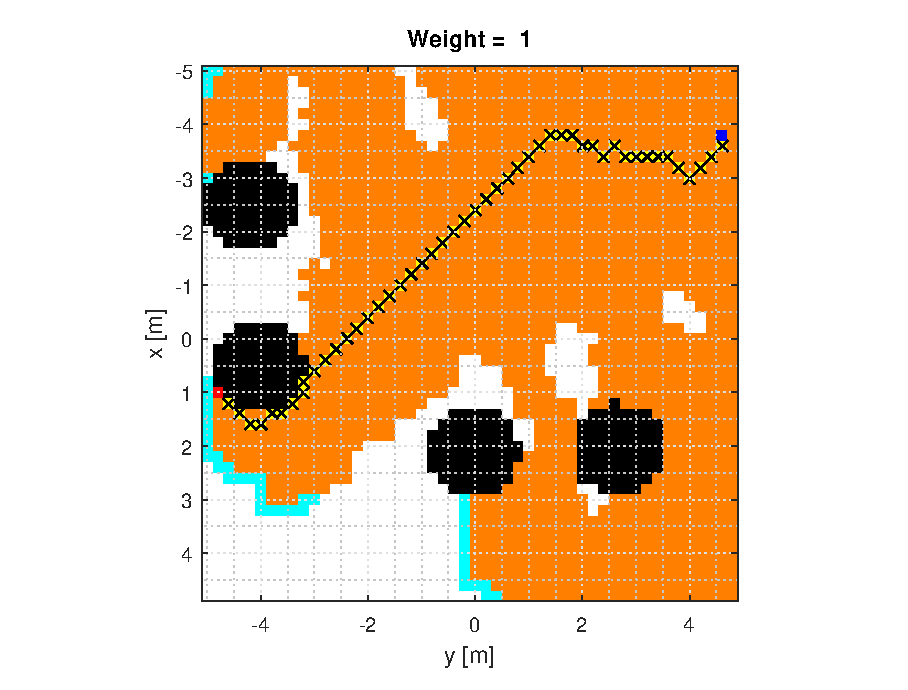
\includegraphics[width = 1\linewidth]{Astar_man_1.eps}
\end{subfigure}
\begin{subfigure}{0.49\linewidth}
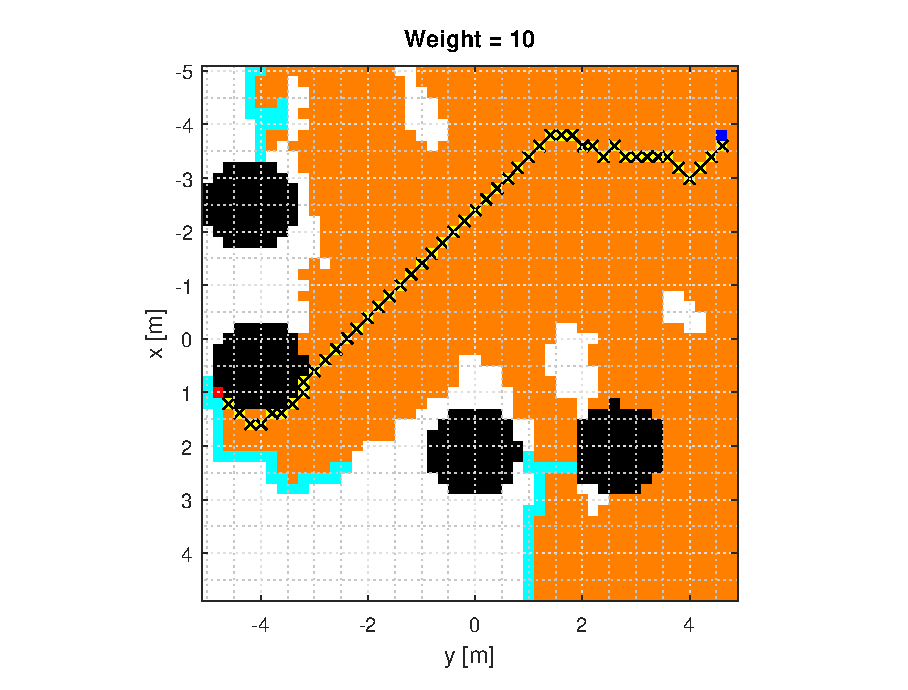
\includegraphics[width = 1\linewidth]{Astar_man_10.eps}
\end{subfigure}
\begin{subfigure}{0.49\linewidth}
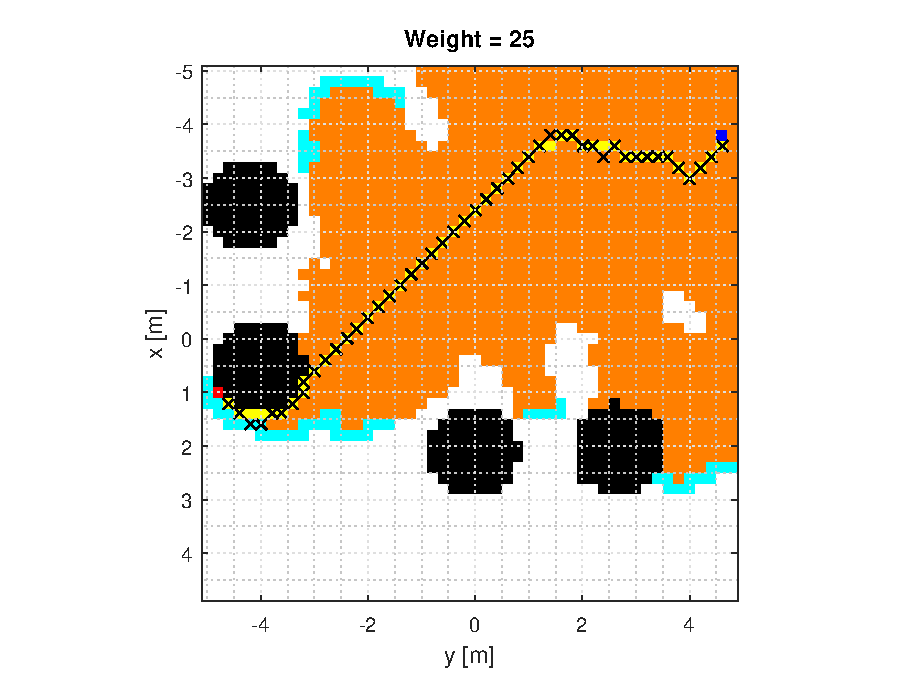
\includegraphics[width = 1\linewidth]{Astar_man_25.eps}
\end{subfigure}
\begin{subfigure}{0.49\linewidth}
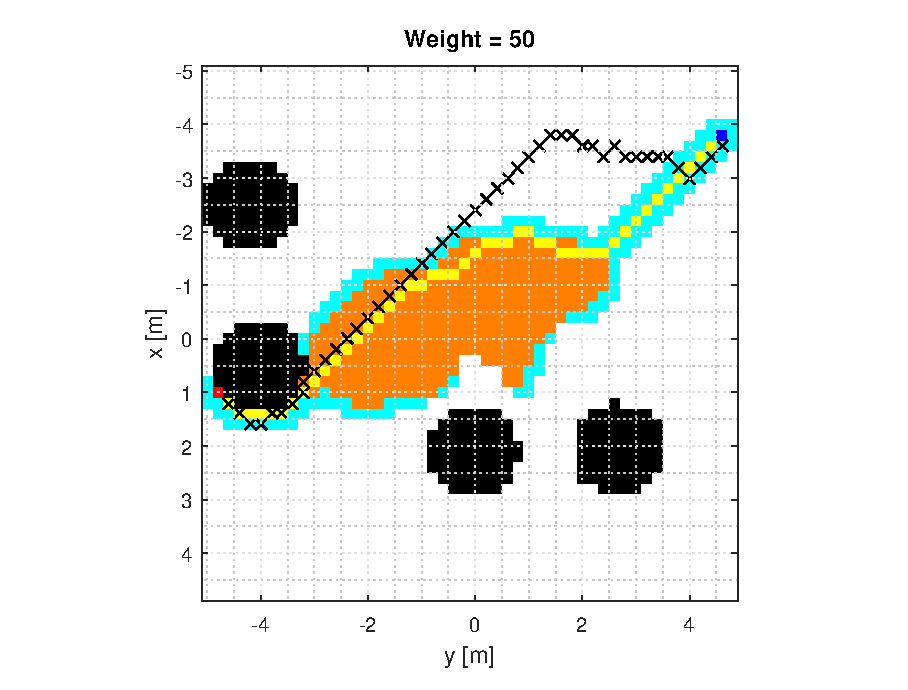
\includegraphics[width = 1\linewidth]{Astar_man_50.eps}
\end{subfigure}
\begin{subfigure}{0.49\linewidth}
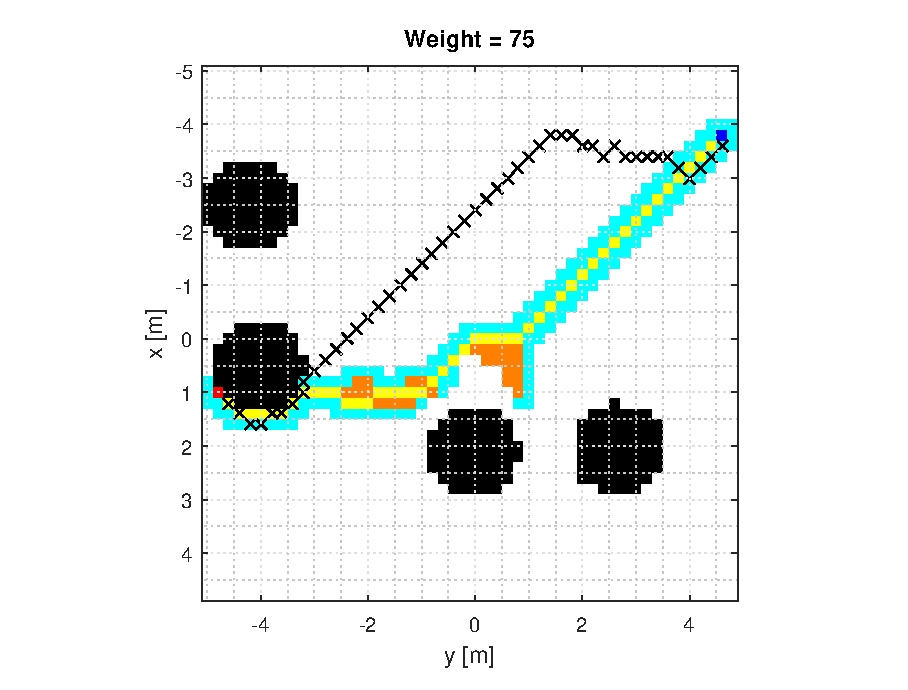
\includegraphics[width = 1\linewidth]{Astar_man_75.eps}
\end{subfigure}
\begin{subfigure}{0.49\linewidth}
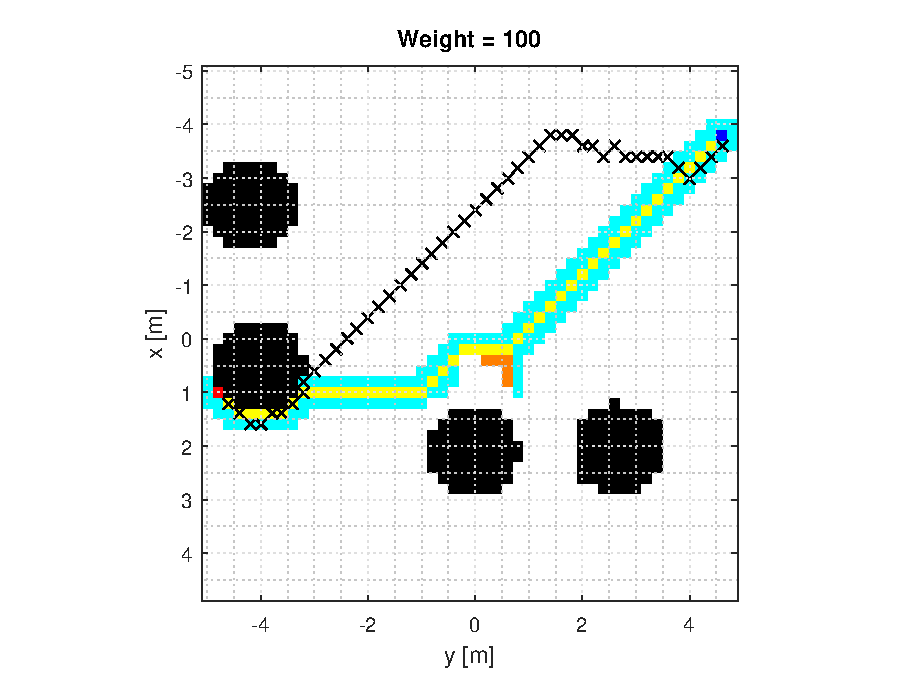
\includegraphics[width = 1\linewidth]{Astar_man_100.eps}
\end{subfigure}
\end{figure}




\end{document}